The details of the numerical setup are presented in Section \ref{f1}.

The main difference is that we no longer use the penalty formulation and therefore 
keep both velocity and pressure as unknowns. Therefore we end up having to solve 
the following system:
\[
\left(
\begin{array}{cc}
\K & \G \\ \G^T & 0 
\end{array}
\right)
\cdot
\left(
\begin{array}{c}
V \\ P
\end{array}
\right)
=
\left(
\begin{array}{c}
 f \\ h
\end{array}
\right)
\quad\quad
{\rm or,}
\quad\quad
\A \cdot X = rhs
\]
Each block $\K$, $\G$ and vector $f$, $h$ are built separately in the code and assembled into 
the matrix $\A$ and vector $rhs$ afterwards. $\A$ and $rhs$ are then passed to the solver. 
We will see later that there are alternatives to solve this approach which do not require to 
build the full Stokes matrix $\A$. 

Each element has $m=4$ vertices so in total $ndofV\times m=8$ velocity dofs and a single 
pressure dof, commonly situated in the center of the element. The total number of 
velocity dofs is therefore $NfemV=nnp \times ndofV$ while the total number of
pressure dofs is $NfemP=nel$. The total number of dofs is then $Nfem=NfemV+NfemP$.

As a consequence, matrix $\K$ has size $NfemV,NfemV$ and matrix $\G$ has size $NfemV,NfemP$.
Vector $f$ is of size $NfemV$ and vector $h$ is of size $NfemP$.  


\fbox{
\parbox{10cm}{{\bf features}
\begin{itemize}
\item $Q_1\times P_0$ element \index{$Q_1 \times P_0$}
\item incompressible flow \index{incompressible flow}
\item mixed formulation \index{mixed formulation}
\item Dirichlet boundary conditions (no-slip)
\item direct solver (?)
\item isothermal \index{isothermal}
\item isoviscous \index{isoviscous}
\item analytical solution \index{analytical solution}
\item pressure smoothing \index{pressure smoothing} 
\end{itemize}
}}

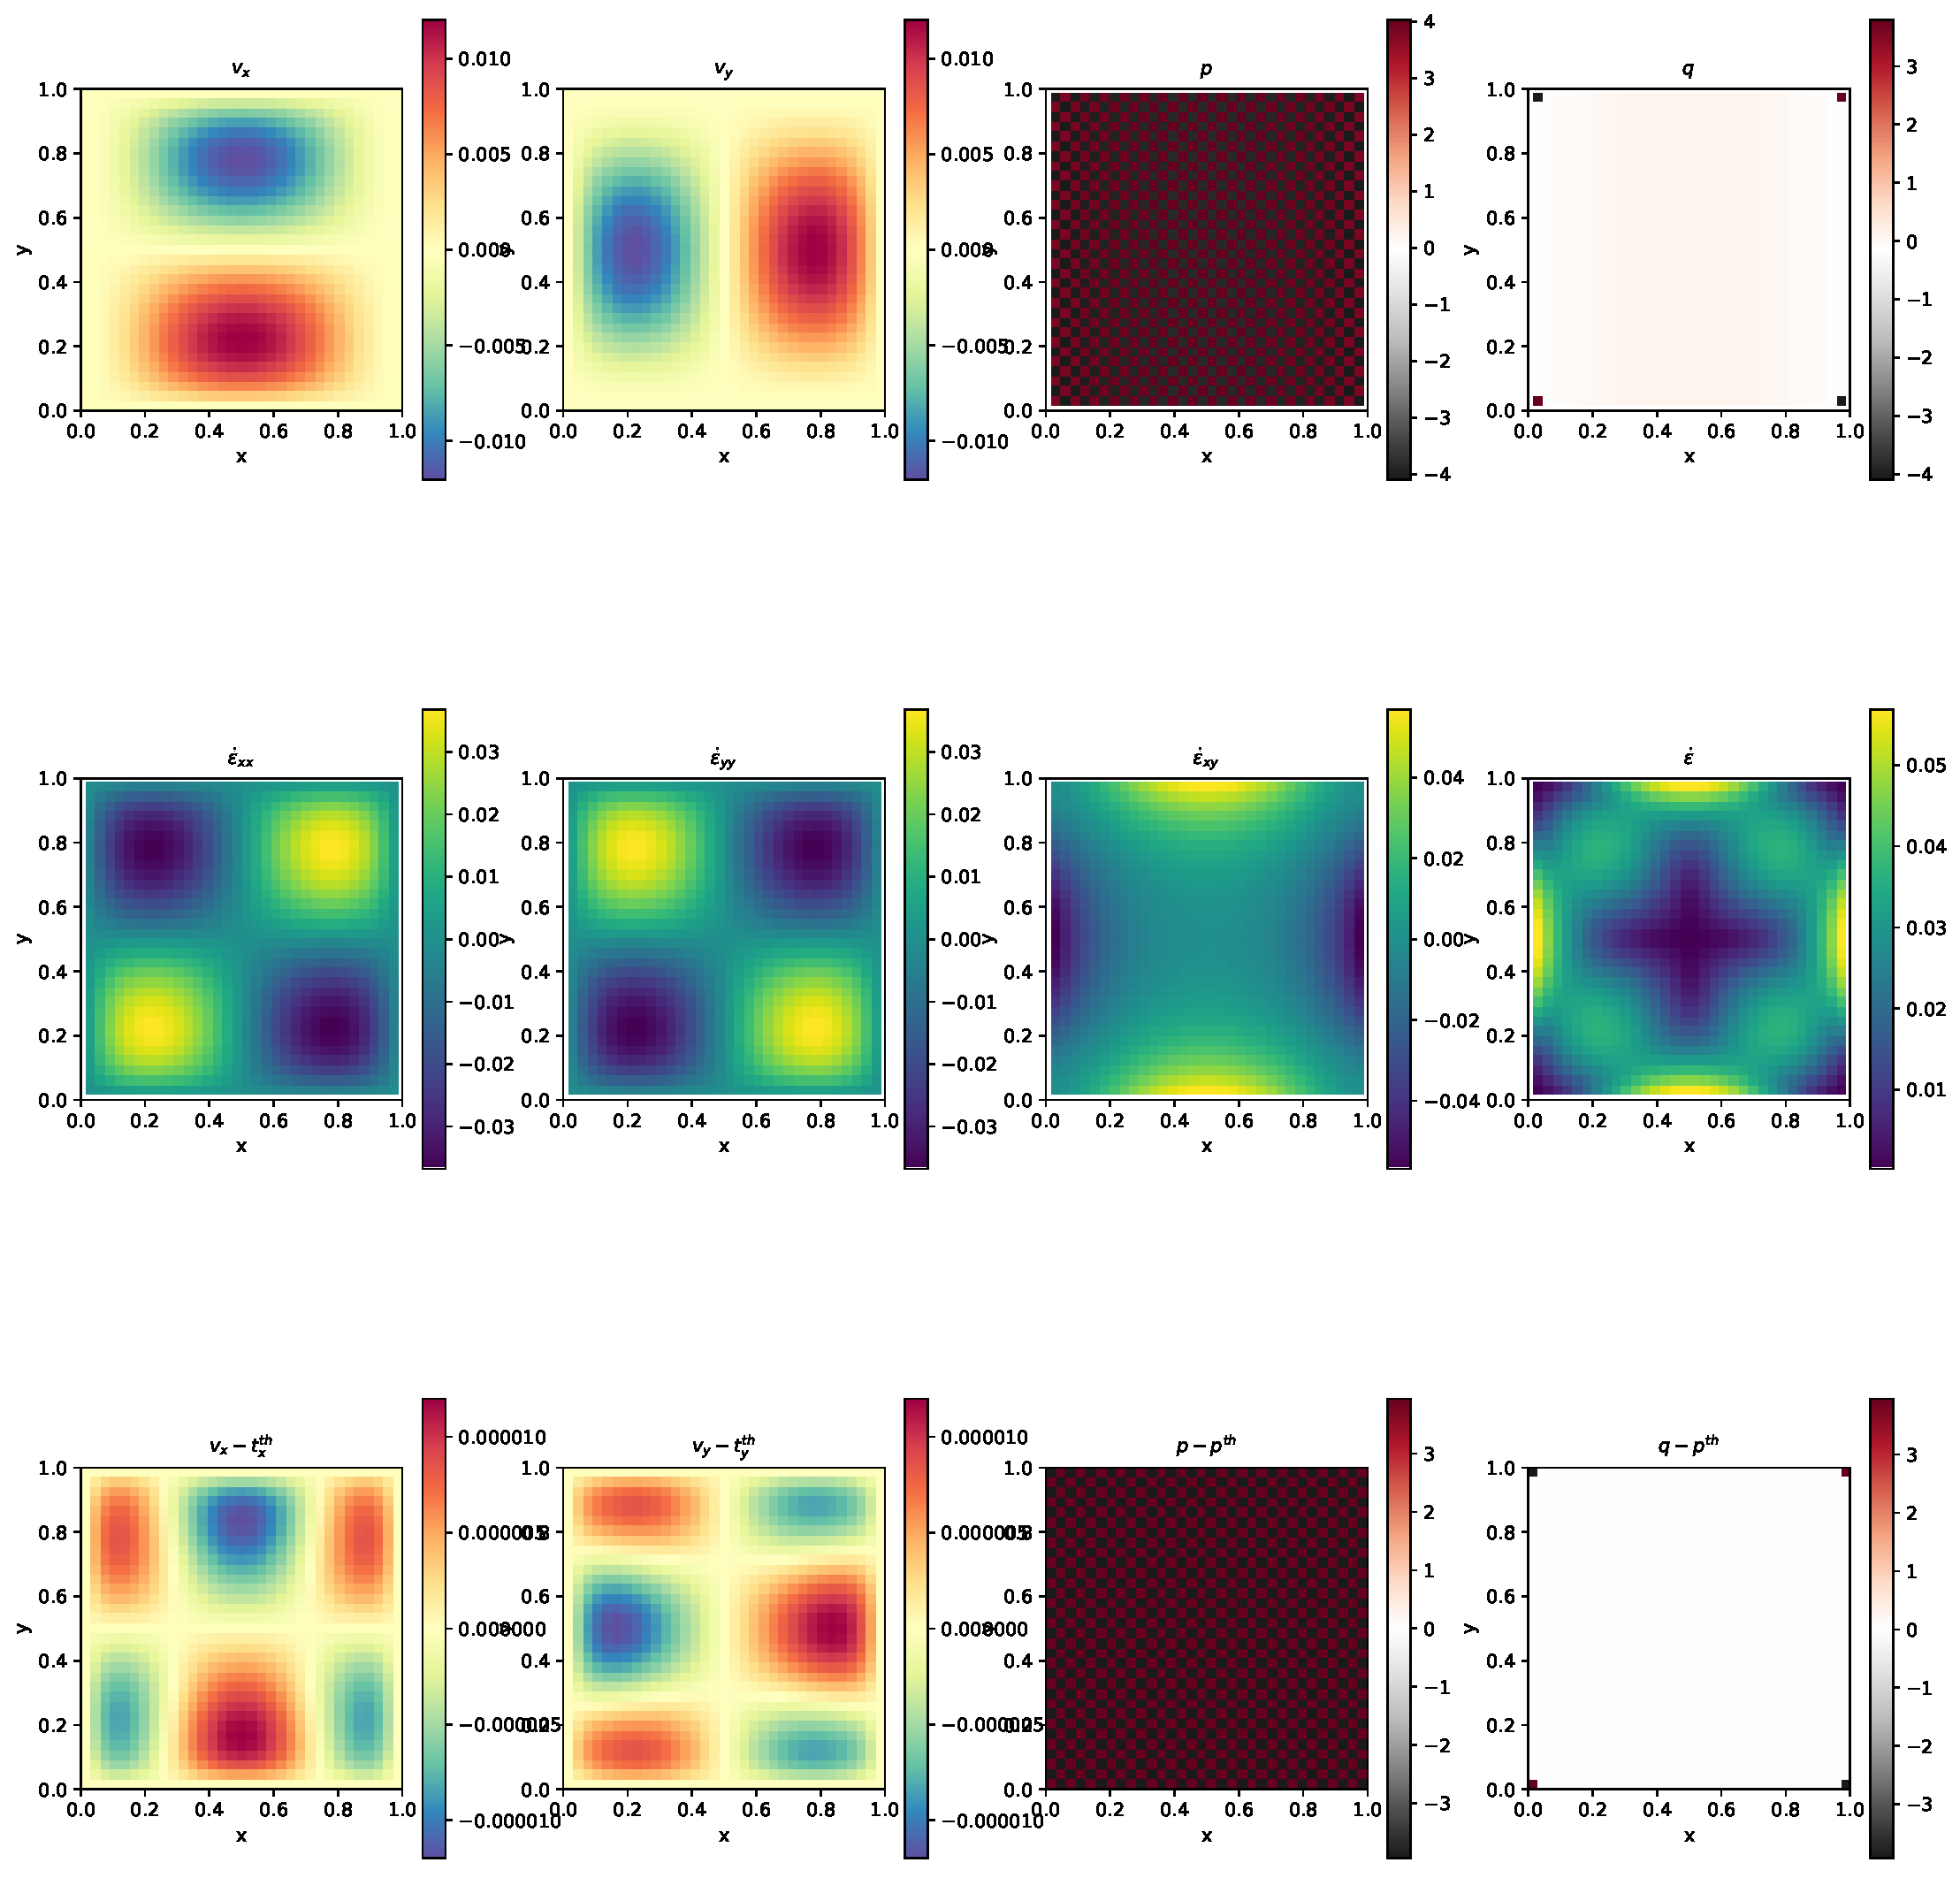
\includegraphics[width=16cm]{python_codes/fieldstone_14/solution.pdf}

Unlike the results obtained with the penalty formualtion (see Section \ref{f1}),
the pressure showcases a very strong checkerboard pattern, similar to the one 
in \cite{dohu05}.

\begin{center}
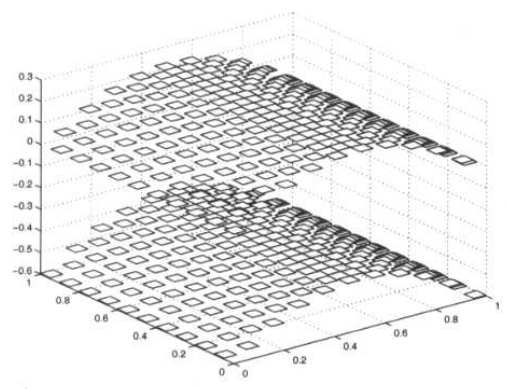
\includegraphics[width=7cm]{python_codes/fieldstone_14/doneahuerta}
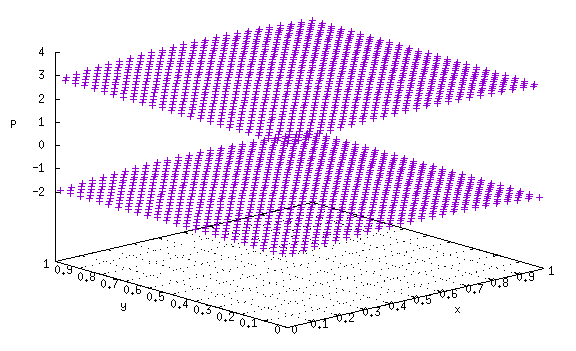
\includegraphics[width=7cm]{python_codes/fieldstone_14/mine}\\
Left: pressure solution as shown in \cite{dohu05}; Right: pressure solution obtained
with fieldstone.
\end{center}

Rather interestingly, the nodal pressure (obtained with a simple center-to-node algorithm)
fails to recover a correct pressure at the four corners.
